% ========== Template by I. Ritter, 2022
% ========== Based on the template of IC\M/T Institute of Creative\Media/Technologies by  M. Wagner and K. Blumenstein, 2016 which is based on the LaTeX Thesis Template for the University of Applied Sciences St.Pölten by P. Lechner https://github.com/hrtlacek/ThesisTemplate-FH-StP        ============= 


%Dokumentklasse without end dot ;-)
\documentclass[a4paper,11pt, numbers=noenddot]{scrreprt}
\usepackage[left= 3.5cm,right = 3cm, bottom = 3.5 cm, top = 3 cm]{geometry}
\usepackage[onehalfspacing]{setspace}

% ============= Settings for the Work =============

\def\workTitle{Identifizierung von Kommunikationsbeziehungen in einem "Enterprise Network"}
\def\subTitle{Expose für eine Bachelorarbeit zum Thema: }
\def\specialization{<IT Security>}
\def\studentFirstName{Mario}
\def\studentLastName{Langmann}
\def\studentId{is201309}
\def\advisorPreTitle{Dipl.\ Ing}
\def\advisoFirstName{Gerald}
\def\advisorLastName{Weinberger}
\def\advisorPosTitle{BSc}
\def\assessorPreTitle{<Pre-Title>}
\def\assessorFirstName{<FirstName>}
\def\assessorLastName{<LastName>}
\def\assessorPosTitle{<Pos-Title>}
\def\place{Steyr}
\def\dateDay{08}
\def\dateMonth{10}
\def\dateYear{2023}
% Switch between German and English version!!! 
\newif\ifuseGermanVersion	% <== DONT TOUCH THIS!!!
% To switch the version please use the comment "%" option :-). After a language change, jou have to rebuild the whole project (in Overleaf --> recompile from scratch) 
\useGermanVersiontrue		% German version
%\useGermanVersionfalse		% English version

% ============= Packages =============

% Dokumentinformationen
\usepackage[
	pdftitle={\workTitle},
	pdfsubject={},
	pdfauthor={\studentFirstName \studentLastName},
	pdfkeywords={}
	pdftex=true, 
	colorlinks=true,
 	breaklinks=true,
	citecolor=black,
	linkcolor=black,	
	menucolor=black,	
	urlcolor=black
]{hyperref}

\hypersetup{
    bookmarks=true,         % show bookmarks bar?
    unicode=false,          % non-Latin characters in Acrobat’s bookmarks
    pdftoolbar=true,        % show Acrobat’s toolbar?
    pdfmenubar=true,        % show Acrobat’s menu?
    pdffitwindow=false,     % window fit to page when opened
    pdfstartview={FitH},    % fits the width of the page to the window
    pdftitle={My title},    % title
    pdfauthor={Author},     % author
    pdfsubject={Subject},   % subject of the document
    pdfcreator={Creator},   % creator of the document
    pdfproducer={Producer}, % producer of the document
    pdfkeywords={keyword1} {key2} {key3}, % list of keywords
    pdfnewwindow=true,      % links in new window
    colorlinks=false,       % false: boxed links; true: colored links
    linkcolor=black,          % color of internal links (change box color with linkbordercolor)
    citecolor=black,        % color of links to bibliography
    filecolor=black,      % color of file links
    urlcolor=black           % color of external links
}

% Standard Packages
\usepackage[utf8]{inputenc}

%For tables
\usepackage{tabularx}

%Text placement
\usepackage{ragged2e}

% Switch the Language
\ifuseGermanVersion
	\usepackage[ngerman]{babel}	% German
\else
	\usepackage[english]{babel} % English
\fi

\usepackage[T1]{fontenc}
\usepackage{graphicx}
\usepackage{graphicx, subfigure}
%setze pfad fuer Bilder
\graphicspath{{img/}}
\usepackage{fancyhdr}
\usepackage{lmodern}
\usepackage{color}
\usepackage{transparent}

% Citation style
\usepackage[
    backend=biber,
    style=numeric,
    isbn=false, 
    %issn=false, 
    doi=false, 
  ]{biblatex}
  
%Add bib source
\addbibresource{Bibliography.bib}

% zusätzliche Schriftzeichen der American Mathematical Society
\usepackage{amsfonts}
\usepackage{mathtools}

\usepackage[export]{adjustbox}

% BlockDiagram Drawing Package
% ---tikz
\usepackage{tikz}
\usetikzlibrary{positioning}
\usepackage{pgfplots}
\pgfplotsset{compat=1.10}
\usepackage{textcomp}

%Package for using the [H] option on graphics to force them into place
\usepackage{float}

%iPython packages:
\usepackage{graphicx} % Used to insert images
\usepackage{adjustbox} % Used to constrain images to a maximum size 
\usepackage{color} % Allow colors to be defined
\usepackage{enumerate} % Needed for markdown enumerations to work
\usepackage{geometry} % Used to adjust the document margins
\usepackage{amsmath} % Equations
\usepackage{amssymb} % Equations
%\usepackage[mathletters]{ucs} % Extended unicode (utf-8) support
% \usepackage[utf8x]{inputenc} % Allow utf-8 characters in the tex document
\usepackage{fancyvrb} % verbatim replacement that allows latex
\usepackage{grffile} % extends the file name processing of package graphics 
                         % to support a larger range 
    % The hyperref package gives us a pdf with properly built
    % internal navigation ('pdf bookmarks' for the table of contents,
    % internal cross-reference links, web links for URLs, etc.)
\usepackage{hyperref}
\usepackage{longtable} % longtable support required by pandoc >1.10

% embedding of audio/video files etc.
% \usepackage{attachfile}
% \usepackage{movie15}
% \usepackage{media9}
% \usepackage{menukeys}

\usepackage[labelfont=it, labelsep=period, format=plain,justification=raggedright, singlelinecheck=false]{caption}
\captionsetup[figure]{justification=centering}
\definecolor{light-gray}{gray}{0.85}

% Switch between German and English based on the Settingx.tex. file
\usepackage{ifthen}

%\captionsetup[listing]{
%  labelsep = newline,
%  textfont = sc, 
%  name = LISTING, 
%  justification=justified,
%  singlelinecheck=false,%%%%%%% a single line is centered by default
%  labelsep=colon,%%%%%%
%  skip = \medskipamount}

% =============== BlockDiagram Drawing Config
\usetikzlibrary{shapes,arrows}

% Definition of blocks:
\tikzset{%
  block/.style    = {draw, thick, rectangle, minimum height = 3em,
    minimum width = 3em},
  sum/.style      = {draw, circle, node distance = 2cm}, % Adder
  input/.style    = {coordinate}, % Input
  output/.style   = {coordinate}, % Output
  mult/.style	  = {draw, isosceles triangle, minimum height=1cm, minimum width =1cm}
}
%mult/.style	  = {isosceles triangle, sharp corners, anchor=center, xshift=-4mm, minimum height=1.5cm, minimum width =0.05cm}
%isosceles triangle, fill=gray!25, minimum width=1.5cm

% Defining string as labels of certain blocks.
\newcommand{\suma}{\Large$+$}
\newcommand{\inte}{$\displaystyle \int$}
\newcommand{\derv}{\huge$\frac{d}{dt}$}
\newcommand{\conv}{\huge$\ast$}

% ============================================

%packages and setings to show colored code
\usepackage{listings}
\usepackage{xcolor}

\definecolor{codegreen}{rgb}{0,0.6,0}
\definecolor{codegray}{rgb}{0.5,0.5,0.5}
\definecolor{codepurple}{rgb}{0.58,0,0.82}
\definecolor{backcolour}{rgb}{0.95,0.95,0.92}

\lstdefinestyle{mystyle}{
    backgroundcolor=\color{backcolour},   
    commentstyle=\color{codegreen},
    keywordstyle=\color{magenta},
    numberstyle=\tiny\color{codegray},
    stringstyle=\color{codepurple},
    basicstyle=\ttfamily\footnotesize,
    breakatwhitespace=false,         
    breaklines=true,                 
    captionpos=b,                    
    keepspaces=true,                 
    numbers=left,                    
    numbersep=5pt,                  
    showspaces=false,                
    showstringspaces=false,
    showtabs=false,                  
    tabsize=2
}

\lstset{style=mystyle}

% Setze arial font
%\usepackage[scaled]{uarial}
%\renewcommand*{\familydefault}{\sfdefault}

% FH-grünBlau
\definecolor{FH}{rgb}{0.10, 0.57, 0.68}
% FH-grünBlau 2
\definecolor{FH2}{rgb}{0.0392, 0.666, 0.549}


% nicht einrücken nach Absatz
\setlength{\parindent}{0pt}

% ============= Kopf- und Fußzeile =============

%\renewcommand{\headrulewidth}{0.4pt}
%\renewcommand{\footrulewidth}{0pt}

\renewcommand{\chaptermark}[1]{\markboth{\thechapter~ #1}{}}

\fancypagestyle{icmt-fancy}{%
  \fancyhf{}% Clear header and footer
  \fancyhead[L]{\leftmark}
  \fancyfoot[R]{\thepage}% Custom footer
  \renewcommand{\headrulewidth}{0.4pt}% Line at the header visible
  \renewcommand{\footrulewidth}{0.0pt}% Line at the footer visible
}

% Redefine the plain page style
\fancypagestyle{plain}{%
  \fancyhf{}%
  \fancyfoot[R]{\thepage}%
  \renewcommand{\headrulewidth}{0pt}% Line at the header invisible
  \renewcommand{\footrulewidth}{0.0pt}% Line at the footer visible
}

% ============= Package Einstellungen & Sonstiges ============= 

%Besondere Trennungen
\hyphenation{De-zi-mal-tren-nung St-rei-fen-licht-scan-nern}

%römische Aufzählungen mit \RM{Zahl}
\newcommand{\RM}[1]{\MakeUppercase{\romannumeral #1}}

% ============= Dokumentbeginn =============

\begin{document}

% Select the right main page ;-)
\ifuseGermanVersion
	
% setup page dimensions for titlepage
\newgeometry{left=2.4cm,right=2.4cm,bottom=2.5cm,top=2cm}

% force baselineskip and parindent
%\newlength{\tmpbaselineskip}
%\setlength{\tmpbaselineskip}{\baselineskip}
%\setlength{\baselineskip}{13.6pt}
%\newlength{\tmpparindent}
%\setlength{\tmpparindent}{\parindent}
%\setlength{\parindent}{17pt}

% first titlepage
\pagestyle{empty}

\begin{figure}[H]
\vspace*{-2.5cm}
\hspace*{2.5cm}

\includegraphics[keepaspectratio, width=1.4\textwidth, right]{TemplateElements/logo_info_sec.png}
\end{figure}



\begin{center}

\vspace{0.5cm}

\begin{minipage}[t][5cm][s]{\textwidth}%
\centering
\LARGE{{{\fontsize{16}{24} \selectfont \subTitle\\}}}
\Huge{{{\fontsize{24}{30} \selectfont \workTitle\\}}}
\vspace{0.5cm}

\end{minipage}

\vspace{0.5cm}

\vspace{1cm}

eingereicht von:\\ 
\fontsize{15pt}{15pt}\selectfont
\textbf{\studentFirstName\ \studentLastName} \\
\fontsize{11pt}{15pt}\selectfont
\studentId

\vspace{1cm}

im Rahmen des Studiengangs\\ 
\textbf{IT Security} 

\vspace{1.8cm}

\begin{tabular}{lll}
Betreuer: & \advisorPreTitle\ \advisoFirstName\ \advisorLastName, \advisorPosTitle\\
\end{tabular}

\vspace{1.8cm}

%\vspace{5cm}
%\begin{tabularx}{\textwidth}[b]{p{5cm} X p{5cm}} \cline{1-1} \cline{3-3}
%Unterschrift Autor:in & & Unterschrift Betreuer:in
%\end{tabularx}

\begin{table}[h]
\centering
\begin{tabular}{lll}
\place, \dateDay.\dateMonth.\dateYear
% & \hrulefill                  & \hrulefill                     \\
%      & Unterschrift Autor:in & Unterschrift Betreuer:in
\end{tabular}
\end{table}

\end{center}

\restoregeometry
\else
	% setup page dimensions for titlepage
\newgeometry{left=2.4cm,right=2.4cm,bottom=2.5cm,top=2cm}

% force baselineskip and parindent
%\newlength{\tmpbaselineskip}
%\setlength{\tmpbaselineskip}{\baselineskip}
%\setlength{\baselineskip}{13.6pt}
%\newlength{\tmpparindent}
%\setlength{\tmpparindent}{\parindent}
%\setlength{\parindent}{17pt}

% first titlepage
\pagestyle{empty}

\begin{figure}[H]
\vspace*{-2.5cm}
\hspace*{2.5cm}

\includegraphics[keepaspectratio, width=1.4\textwidth, right]{TemplateElements/logo_info_sec.png}
\end{figure}



\begin{center}

\vspace{0.5cm}

\begin{minipage}[t][5cm][s]{\textwidth}%
\centering
\Huge{{{\fontsize{24}{30} \selectfont \workTitle\\}}}
\vspace{0.5cm}
\LARGE{{{\fontsize{16}{24} \selectfont \subTitle\\}}}
\end{minipage}

\vspace{0.5cm}


\LARGE{Bachelor's thesis}


\vspace{1cm}

\fontsize{11pt}{15pt}\selectfont for the attainment of the academic degree\\
\textbf{Bachelor of Science in Engineering (BSc)}

\vspace{1cm}

submitted by:\\ 
\fontsize{15pt}{15pt}\selectfont
\textbf{\studentFirstName\ \studentLastName} \\
\fontsize{11pt}{15pt}\selectfont
\studentId

\vspace{1cm}

as part of the study programme\\ 
\textbf{Data Science and Business Analytics} 

\vspace{1.8cm}

\begin{tabular}{lll}
Supervisor and first assessor: & \advisorPreTitle\ \advisoFirstName\ \advisorLastName, \advisorPosTitle\\
Second assessor: & \assessorPreTitle\ \assessorFirstName\ \assessorLastName, \assessorPosTitle\\
\end{tabular}

\vspace{1.8cm}

%\vspace{5cm}
%\begin{tabularx}{\textwidth}[b]{p{5cm} X p{5cm}} \cline{1-1} \cline{3-3}
%Unterschrift Autor:in & & Unterschrift Betreuer:in
%\end{tabularx}

\begin{table}[h]
\centering
\begin{tabular}{lll}
\place, \dateDay.\dateMonth.\dateYear
 & \hrulefill                  & \hrulefill                     \\
      & Signature author & Signature assessor
\end{tabular}
\end{table}

\end{center}

\restoregeometry
\fi

% \part im Inhaltsverzeichnis nicht nummerieren
\makeatletter
\let\partbackup\l@part
\renewcommand*\l@part[2]{\partbackup{#1}{}}

%Seitennummerierung neu beginnen, Zahlen [arabic], röm.Zahlen [roman,Roman], Buchstaben [alph,Alph]
\pagenumbering{Roman}

\newpage
%\ifuseGermanVersion
%	\chapter*{Ehrenwörtliche Erklärung}
\label{ch:erklaerung}
% \begin{justify}
% 	test
% \end{justify}

Ich versichere, dass 

\begin{justify}
- ich diese Bachelorarbeit selbständig verfasst, andere als die angegebenen Quellen und Hilfsmittel nicht benutzt und mich sonst keiner unerlaubten Hilfe bedient habe.
\end{justify}

\begin{justify}
- ich dieses Bachelorarbeitsthema bisher weder im Inland noch im Ausland einem Begutachter/ einer Begutachterin zur Beurteilung oder in irgendeiner Form als Prüfungsarbeit vorgelegt habe.	
\end{justify}

\begin{justify}
- diese Arbeit mit der vom Begutachter/von der Begutachterin beurteilten Arbeit übereinstimmt. 
\end{justify}
% - diese Arbeit mit der vom Begutachter/von der Begutachterin beurteilten Arbeit übereinstimmt. \\
% \\[1.5cm]

\begin{justify}
Der Studierende/Absolvent räumt der FH St. Pölten das Recht ein, die Bachelorarbeit für Lehre- und Forschungstätigkeiten zu verwenden und damit zu werben (z.B. bei der Projektevernissage, in Publikationen, auf der Homepage), wobei der Absolvent als Urheber zu nennen ist. Jegliche kommerzielle Verwertung/Nutzung bedarf einer weiteren Vereinbarung zwischen dem Studierenden/Absolventen und der FH St. Pölten. \\[1.5cm]	
\end{justify}

Datum:	\hrulefill\enspace Unterschrift Autor:in: \hrulefill
\\[3.5cm]
%\else
%	\chapter*{Declaration}
\label{ch:declaration}

I hereby declare that

\begin{justify}
- the attached research paper is my own, original work undertaken in partial fulfillment of my degree.
\end{justify}

\begin{justify}
- I have made no use of sources, materials or assistance other than those which habe been openly and fully acknowledged in the text. If any part of another person’s work has been quoted, this either appears in inverted commas or (if beyond a few lines) is indented.
\end{justify}

\begin{justify}
- any direct quotation or source of ideas has been identified in the text by author, date, and page number(s) immediately after such an item, and full details are provided in a reference list at the end of the text.
\end{justify}

\begin{justify}
- I understand that any breach of the fair practice regulations may result in a mark of zero for this research paper and that it could also involve other repercussions.
\end{justify}

\begin{justify}
The student/graduate grants the St. Pölten  University of Applied Sciences the right to use the bachelor's thesis for teaching and research activities and to advertise it (e.g. at the project vernissage, in publications, on the homepage), whereby the graduate is to be named as the author. Any commercial exploitation/use requires a further agreement between the student/graduate and St. Pölten University of Applied Sciences. \\[1.5cm]
\end{justify}

Date:	\hrulefill\enspace Signature: \hrulefill
\\[3.5cm]
%\fi

%\newpage
%%\chapter*{Kurzfassung}
%\label{ch:kurzfassung}
%Dies ist die Kurzfassung der Arbeit. Lorem ipsum dolor sit amet, consectetur adipisicing elit, sed do eiusmod
%tempor incididunt ut labore et dolore magna aliqua. Ut enim ad minim veniam,
%quis nostrud exercitation ullamco laboris nisi ut aliquip ex ea commodo
%consequat. Duis aute irure dolor in reprehenderit in voluptate velit esse
%cillum dolore eu fugiat nulla pariatur. Excepteur sint occaecat cupidatat non
%proident, sunt in culpa qui officia deserunt mollit anim id est laborum.


%\newpage

\chapter*{Abstract}
\label{ch:abstract}

Introduction: Warum behandeln wir das Thema

Purpose: Welches Problem soll gelöst werden

Method: Wie wurde die Problemlösung gemacht

Product: Was war das Ergebnis

Conclusion: Was sind die Folgerungen / Schlussfolgerungen aus den gewonnen Erkenntnissen

keine Referenzen und Zitate


%\chapter*{Kurzfassung}
\label{ch:kurzfassung}

Das Abstract auf deutsch.

%\newpage

%Inhaltsverzeichnis
\tableofcontents

\newpage
%Seitennummerierung neu beginnen, Zahlen [arabic], röm.Zahlen [roman,Roman], Buchstaben [alph,Alph]
\pagenumbering{arabic}

% pagestyle für gesamtes Dokument aktivieren
\pagestyle{icmt-fancy}
\newpage

% /*================================
% =            EXAMPLE            =
% ================================*/

% Delete this include at the end
%\chapter{Example}
\label{ch:example}

!!! Please delete this chapter after finishing your work !!!

\section{Settings}

To add your name and the title of your work, please use the ``Settings.tex'' file!
Additionally, switch there between German and English version.

\section{How to Make Sections and Subsections}

Use section and subsection commands to organize your document. \LaTeX{} handles all the formatting and numbering automatically. Use ref and label commands for cross-references.

\subsection{How to Make Lists}

You can make lists with automatic numbering \dots

\begin{enumerate}
\item Like this,
\item and like this.
\end{enumerate}
\dots or bullet points \dots
\begin{itemize}
\item Like this,
\item and like this.
\end{itemize}
\dots or with words and descriptions \dots
\begin{description}
\item[Word] Definition
\item[Concept] Explanation
\item[Idea] Text
\end{description}\section{Section}

You have to write text between each headline.

\section{Citation}

This part describes the 3 types of citations which are possible:

\section{Direct Citation}

The maximum for a direct citation is a ${1/2}$ page.

\begin{quote}
    "Cite"\cite{Verma.2021}
\end{quote}

\section{Floating Text Citation}

He defined the Visual Information Seeking Mantra as ``Overview first, zoom and filter, then details-on-demand''.\cite{Verma.2021}

\section{Indirect Citation}

Some text which summarizes a paper or a book chapter. This could take several lines.\cite{Verma.2021}. 

\section{Tools}

There are many tools that help with literature management and knowledge organization. Citavi, Zotero and Co. are just a few of them.\\

Citavi: \url{https://www.citavi.com/de}\\
Zotero: \url{https://www.zotero.org/}

\newpage
\section{Figures}

To place a figure use the following code example

\begin{figure}[ht!]
  \centering
  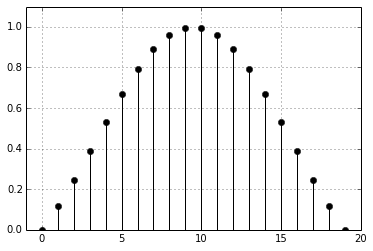
\includegraphics[width=1\columnwidth]{Figures/Example}
  \caption{Interactive data exploration with multiple devices.}
  \label{fig:example}
\end{figure}

Refer to a figure in the following forms:\\
If you take a look at Figure~\ref{fig:example} ...\\
... text text (see Figure~\ref{fig:example}) ...

\section{Listings}
\begin{lstlisting}[language= Python, caption={Funktion.}\label{funk},captionpos=b]
def tokenize(text):
    result = []
    for token in gensim.utils.simple_preprocess(text):
        if token not in stop_words \
                and len(token) > 2:  # drops words with less than 3 characters
            result.append(lemmatize(token))
    return result
\end{lstlisting}

Ok, Now lets take a look at Listing~\ref{funk}.

\newpage
\section{Table}

\begin{table}[ht!]
  \caption{My caption with a very useful description. die kann auch etwas länger sein und über mehrere Zeilen gehen und so weiter.}
  \label{my-label}
  \begin{tabular}{llr}
    \hline
    \multicolumn{2}{c}{Item} &            \\ \cline{1-2}
    Animal     & Description & Price (\$) \\ \hline
    Gnat       & per gram    & 13.65      \\
               & each        & 0.01       \\
    Gnu        & stuffed     & 92.50      \\
    Emu        & stuffed     & 33.33      \\
    Armadillo  & frozen      & 8.99       \\ \hline
  \end{tabular}
\end{table}

For the fast generation of tables from Excel use \url{http://www.heise.de/download/excel2latex.html}

For the fast generation of tables in general use
\url{https://www.tablesgenerator.com/}

\section{Equations}

\LaTeX{} is great at typesetting equations. Let $X_1, X_2, \ldots, X_n$ be a sequence of independent and identically distributed random variables with $\text{E}[X_i] = \mu$ and $\text{Var}[X_i] = \sigma^2 < \infty$, and let

$$S_n = \frac{X_1 + X_2 + \cdots + X_n}{n}$$

This was a equation without a label.
      
\begin{equation}
S_n = \frac{1}{n}\sum_{i}^{n} X_i
\label{eq:test}
\end{equation}


This is the reference to equation~\ref{eq:test}.      


denote their mean. Then as $n$ approaches infinity, the random variables $\sqrt{n}(S_n - \mu)$ converge in distribution to a normal $\mathcal{N}(0, \sigma^2)$.




% /*================================
% =            CONTENTS            =
% ================================*/

\newcommand{\ot}{\glqq Operative Technology\grqq{}}
\newcommand{\al}{\glqq Application Landscape\grqq{}}
\newcommand{\so}{\glqq Service Owner\grqq{}}
\newcommand{\lan}{\glqq LAN\grqq{}}
\newcommand{\wan}{\glqq WAN\grqq{}}
\chapter{Problemstellung}
\label{ch:Problemstellung}
Die Kommunikation heutzutage ist stark von den unterschiedlichsten Computernetzen abhängig. Diese Computernetze ermöglichen es Menschen und Geräten zu kommunizieren, egal wo sie sich befinden.
\\
Grundsätzlich werden diese Netze in \glqq Lokale Netze(LAN)\grqq{} und \glqq Nichtlokale Netze(WAN)\grqq{} unterschieden. Während wir in der täglichen Kommunikation via Messenger oder E-Mail hauptsächlich über \wan-Netze kommunizieren erfolgt die Kommunikation innerhalb von Produktionsanlagen heute nach wie vor hauptsächlich im \lan. Im Zuge der Arbeit berücksichtigen wir die unterschiedlichsten Typen vom Kommunikationsnetzen, relevant ist aber hauptsächlich die Kommunikation im \lan.
\\
Im Zuge eines globalen angelegten Projektes zur Netzwerksegmentierung sind alle \so{} in \ot{}-Netzen damit konfrontiert die Kommunikationsbeziehungen auf ihre Systeme zu identifizieren und entsprechend auf ihre Notwendigkeit zu bewerten. Durch Anreicherung der identifizierten Daten mit zusätzlichen Datenquellen wie ITSM, DNAC, Firewall – Logs soll es dem AO ermöglicht werden die Kommunikationsbeziehungen seiner Systeme zu identifizieren.
Durch die Verknüpfung der erfassten Daten aller AO soll eine “Application Landscape” für den kompletten Konzern dargestellt werden. 

\chapter{Zielsetzung}
\label{ch:Zielsetzung}
In einem global agierenden Konzern gibt es eine Vielzahl von \so, die für die Verwaltung und Bereitstellung von IT-Services verantwortlich sind. Jeder Service Owner ist für ein bestimmtes System oder eine bestimmte Gruppe von Systemem verantwortlich.
Das Ziel dieser Arbeit ist es, herauszufinden, welche Informationen über die Kommunikationsbeziehungen der Systeme des \so{}  mit den Standardtools eines Betriebssystems (Windows, Linux, MacOS) erfasst werden können und welche konzernweiten Tools dem \so zur Verfügung stehen um die um die bereits recherchierten Informationen weiter anzureichen.\\
Die erfassten Daten der einzelnen Service Owner sollen in einer \al zusammengeführt und entsprechend visualisiert werden.

\chapter{Forschungsstand}
\label{ch:Forschungsstand}

\chapter{Konzept}
\label{ch:Konzept}


\chapter{Gliederung}
\label{ch:Gliederung}



\pagestyle{plain} 

%Literaturverzeichnis
\printbibliography

% Bilderverzeichnis
%\newpage
%\listoffigures
% Tableverzeichnis
%\newpage
%\listoftables
%Codelistingsverzeichnis
%\newpage
%\lstlistoflistings
%\newpage

% ============================================


\chapter*{Appendices}

\addcontentsline{toc}{chapter}{Appendices}
\renewcommand{\thesection}{\Alph{section}}

\section{Appendix}
\label{appendix_a}

LoHrem ipsum dolor sit amet, consectetur adipisicing elit, sed do eiusmod
tempor incididunt ut labore et dolore magna aliqua. Ut enim ad minim veniam,
quis nostrud exercitation ullamco laboris nisi ut aliquip ex ea commodo
consequat. Duis aute irure dolor in reprehenderit in voluptate velit esse
cillum dolore eu fugiat nulla pariatur. Excepteur sint occaecat cupidatat non
proident, sunt in culpa qui officia deserunt mollit anim id est laborum.LoHrem ipsum dolor sit amet, consectetur adipisicing elit, sed do eiusmod
tempor incididunt ut labore et dolore magna aliqua. Ut enim ad minim veniam,
quis nostrud exercitation ullamco laboris nisi ut aliquip ex ea commodo
consequat. Duis aute irure dolor in reprehenderit in voluptate velit esse
cillum dolore eu fugiat nulla pariatur. Excepteur sint occaecat cupidatat non
proident, sunt in culpa qui officia deserunt mollit anim id est laborum.
LoHrem

\newpage

\section{Appendix}
\label{appendix_b}

LoHrem ipsum dolor sit amet, consectetur adipisicing elit, sed do eiusmod
tempor incididunt ut labore et dolore magna aliqua. Ut enim ad minim veniam,
quis nostrud exercitation ullamco laboris nisi ut aliquip ex ea commodo
consequat. Duis aute irure dolor in reprehenderit in voluptate velit esse
cillum dolore eu fugiat nulla pariatur. Excepteur sint occaecat cupidatat non
proident, sunt in culpa qui officia deserunt mollit anim id est laborum.LoHrem ipsum dolor sit amet, consectetur adipisicing elit, sed do eiusmod
tempor incididunt ut labore et dolore magna aliqua. Ut enim ad minim veniam,
quis nostrud exercitation ullamco laboris nisi ut aliquip ex ea commodo
consequat. Duis aute irure dolor in reprehenderit in voluptate velit esse
cillum dolore eu fugiat nulla pariatur. Excepteur sint occaecat cupidatat non
proident, sunt in culpa qui officia deserunt mollit anim id est laborum.
LoHrem


% ============================================

\end{document}























